\documentclass{siproblemset}

\usepackage{multicol}
\usepackage{xcolor}
\usepackage{mathtools}

% SI Session Information
\course{MTH 1321}
\sessionnum{PT3}
\sessiondate{4/5/21}

% Worksheet Information
\title{Practice Test \#3}
\sections{Chapter 4 + 3.10}
\withnamespace

\definecolor{darkred}{RGB}{110,0,0}

%\debugmode

\begin{document}
    \maketitle
    
    \begin{center}
        \framebox{
            \begin{minipage}{\textwidth}
                \begin{center}
                    \textbf{When completing this practice test, do your best to mimic the test environment:}
                \end{center}
                \begin{enumerate}
                    \item Do not use a calculator.
                    \item Try not to use your notes.
                    \item Time yourself, make sure you are completing the problems at a comfortable pace. Remember that you will only get 75 minutes for the actual exam (with fewer questions of course).
                \end{enumerate}
                \begin{center}
                    \color{darkred}\textbf{ Please do not share this practice test with anyone else.\\ \underline{Your} commitment to SI and reviewing material earned this, not anyone else's.}
                \end{center}
                {\centering When you have finished the practice test, check Canvas to check your answers.\\}
            \end{minipage}
        }
    \end{center}
    
    % Approximations and Linearizations 
    \hspace{-5mm}\textbf{Approximations and Linearizations}
    \begin{multipartquestion}
        Information about $f(x)$ and $f'(x)$ is given in the chart below for certain values of $x$.
        
        \begin{center}
            \begin{tabular}{|c|c|c|c|c|}
                \hline
                $x$ & $-2$ & $-1$ & $0$ & $1$\\
                \hline
                $f(x)$ & 3 & 2 & 0 & -1 \\
                \hline
                $f'(x)$ & $-1/8$ & $-1/3$ & $-1$ & $0$\\
                \hline
            \end{tabular}
        \end{center}
    
        \frq{Determine the linearization of $f(x)$ at $x=-1$.}
        \Smallsp
        \frq{Use your answer from part (a) to estimate $f\left(-\dfrac32\right)$.}
    \end{multipartquestion}
    \newpage
    \frq{Approximate the difference $3.01^2-3^2$ using a linear approximation.}
    \largesp

    % Derivative Properties
    \hspace{-5mm}\textbf{Derivative Properties}
    % FIN-F17 2
    \mcq{Suppose $f'(a)=0$. Mark each of the following statements as true (T) (meaning ``\textit{must} be true'') or false (F) (meaning ``\textit{could} be false''). You do \textit{not} need to justify your answer.}{
        \task $f$ is continuous at $x=a$.
        \task The line tangent to $y=f(x)$ at $x=a$ is horizontal.
        \task $f$ has a local max or local min at $x=a$.
        \task $\lim\limits_{x\to a}\dfrac{f(x)-f(a)}{x-a}=0$
        \task $f$ has an inflection point at $x=a$.
        \task $f'$ is continuous at $x=a$.
        \task $x=a$ is a critical value of $f$.
        \task The line tangent to $y=f'(x)$ at $x=a$ is horizontal.
        \task $\lim\limits_{h\to 0}\dfrac{f(x+h)-f(x)}{h}=0$
         
    }
\newpage
    % FIN-F17 8 (modified)
    \mcq{Let $f(x)=x^3+4x^2$}{
        \task Find the intervals on which $f$ is increasing/decreasing.
        \smallsp
        \task Find and classify all local extrema of $f$.
        \smallsp
        \task Find the intervals on which $f$ is concave up/down.
        \smallsp
        \task Find all inflection points of $f$.
        \smallsp
    }
    % FIN-F18 4
%    \begin{multipartquestion}
%        Researchers are studying the effectiveness of a new antibiotic. Let $P(t)$ be the number of bacteria present $t$ hours after the antibiotic is administered. Data collected by the researchers indicated that the over the first $12$ hours, the number of bacteria decreased while its rate of change increased, and then afterwards the number of bacteria continued to decrease, but its rate of change decreased.
%        \mcq{Which first derivative statements best describe this scenario?}{
%            \task $P'(t) > 0$ for $0 < t < 12$ and $P'(t) > 0$ for $t > 12$
%            \task $P'(t) > 0$ for $0 < t < 12$ and $P'(t) < 0$ for $t > 12$
%            \task $P'(t) < 0$ for $0 < t < 12$ and $P'(t) > 0$ for $t > 12$
%            \task $P'(t) < 0$ for $0 < t < 12$ and $P'(t) < 0$ for $t > 12$
%            \task None of the above
%        }
%        \mcq{Which second derivative statements best describe this scenario?}{
%            \task $P''(t) > 0$ for $0 < t < 12$ and $P''(t) > 0$ for $t > 12$
%            \task $P''(t) > 0$ for $0 < t < 12$ and $P''(t) < 0$ for $t > 12$
%            \task $P''(t) < 0$ for $0 < t < 12$ and $P''(t) > 0$ for $t > 12$
%            \task $P''(t) < 0$ for $0 < t < 12$ and $P''(t) < 0$ for $t > 12$
%            \task None of the above
%        }
%        \mcq{At $t=12$, the graph of $y=P(t)$ has}{
%            \task a local maximum
%            \task a local minimum
%            \task a critical number but no local extremum
%            \task an inflection point
%            \task None of the above
%        }
%        \frq{Assuming that there are a positive number of bacteria, $P_0$, present at time $t = 0$ and that at time $t = 24$, all bacteria are eliminated, sketch a possible graph of $P$ corresponding to all the criteria described above.}
%    \end{multipartquestion}
    % FIN-S19 11
%    \begin{multipartquestion}
%        The function $f$ is continuous for all values of $x$. Information about the sign of $f'$ and $f''$ is organized in the table below.
%        
%        \begin{center}
%            \begin{tabular}{|c|c|c|c|c|}
%                \hline
%                &$x<1$&$1<x<2$&$2<x<3$&$x>3$\\
%                \hline
%                Sign of $f'$&$-$&$-$&$+$&$-$\\
%                \hline
%                Sign of $f''$&$+$&$-$&$-$&$+$\\
%                \hline
%            \end{tabular}
%        \end{center}
%    
%        Mark each of the following statements as true (T) or false (F). You do \textit{not} need to justify your answer.
%        \frq{$f$ has a local minimum at $x=2$}
%        \frq{$f$ is decreasing and concave down at $x=4$}
%        \frq{$f$ has an inflection point at $x=1$}
%        \frq{$f'$ is decreasing at $x=2.5$}
%        \frq{$f'$ has a local extremum at $x=1$}
%    \end{multipartquestion}
\newpage
    % REC-10 1
    \begin{multipartquestion}
        For the graph below, determine the following. Assume the domain of $f(x)$ is all real numbers.
        \begin{center}
            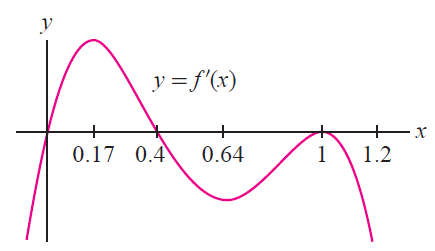
\includegraphics[width=8cm]{ShapeOfGraph}
        \end{center}
        \frq{$f(x)$ is increasing on:}
        \tinysp
        \frq{$f(x)$ is decreasing on:}
        \tinysp
        \frq{$x$-coordinates of local minima}
        \tinysp
        \frq{$x$-coordinates of local maxima}
        \tinysp
        \frq{$f(x)$ is concave up on:}
        \tinysp
        \frq{$f(x)$ is concave down on:}
        \tinysp
        \frq{$x$-coordinates of points of inflection:}
        \tinysp
    \end{multipartquestion}
\newpage
    % REC-10 3
    \begin{multipartquestion}
        \frq{Consider a function $f(x)$ with continuous second derivative. If $f'(2)=0$ and $f''(2)=0$, can we tell if $f$ has a local extrema at $x=2$? If so, is it a maximum or a minimum and why?}
        \Tinysp
        \frq{Consider a function $f(x)$ with continuous second derivative. If $f'(7)=0$ and $f''(7)<0$, can we tell if $f$ has a local extrema at $x=7$? If so, is it a maximum or a minimum and why?}
        \Tinysp
        \frq{Consider a function $f(x)$ with continuous second derivative. If $f'(-3)=0$ and $f''(-3)>0$, can we tell if $f$ has a local extrema at $x=-3$? If so, is it a maximum or a minimum and why?}
        \Tinysp
    \end{multipartquestion}
    % UGA-F18-3 1
    \frq{If applicable, use the Extreme Value Theorem to determine the absolute maximum and minimum values of the function on the given interval. Be sure to justify your use of the Extreme Value Theorem.}
    $$f(x)=\sin(x)-\cos(x)\text{    on the interval }[0,\pi]$$
\newpage
    
    % FIN-F18 7
    \mcq{Suppose $f'(x)=x(x-1)^2$.}{
        \task Find the $x$-coordinate for all local extrema of $f$. Classify each as where a local max or local min occurs.
        \Normalsp
        \task Find the $x$-coordinate for all inflection points of $f$.
        \Normalsp
    }
    % Mean Value Theorem
    \hspace{-5mm}\textbf{Mean Value Theorem}
    % FIN-F17 11
    \frq{Consider $f(x)=x-\dfrac1x$ on $1\leq x\leq 2$. Find a value of $c$ guaranteed by the Mean Value Theorem.}
    \newpage
    
%    % Optimization
%    \hspace{-5mm}\textbf{Optimization}
%    \frq{A rectangle is inscribed in the first quadrant region bounded by the $x$-axis, the $y$-axis, and the parabola $y=16-x^2$. That is, the base of the rectangle is along the $x$-axis, its lower left corner is at the origin, and its upper right corner is on the parabola $y=16-x^2$. Find the length and width of the rectangle of greatest perimeter.}
%    \hugesp
%    \frq{We want to construct a box whose base length is 3 times the base width. The material used to build the top and bottom cost \$5 per square foot and the material used to build the sides cost \$4 per square foot. If the box must have a volume of $50$ cubic feet, determine the dimensions that will minimize the cost to build the box.}
%    \hugesp
%    \frq{Find the points on the graph $y=4-2x^2$ that are closest to $(0,-4)$. Hint: remember that the distance between the points $(x,y)$ and $(a,b)$ is $d=\sqrt{(x-a)^2+(y-b)^2}$. \textbf{Also remember that minimizing $d$ is the same as minimizing $d^2$.}}
%    \hugesp
%    \frq{Find the maximum volume of a cylinder whose surface area is $300\pi$ square meters.}
%    \newpage
    
    % Miscellaneous
    \hspace{-5mm}\textbf{Miscellaneous}
    
    \begin{multipartquestion}
        You begin to heat a pot of water on the stove. At time $t$ (in minutes), the temperature $T$ (in $^{\circ}$F) of the water is recorded below. For $0 \leq t \leq 8$, $T$ is a differentiable function of $t$.
        \begin{center}
            \begin{tabular}{|l|r|r|r|r|r|}
                \hline
                $t$ (min) & 0 & 1 & 3 & 4 & 8 \\
                \hline
                $T$ ($^{\circ}$F) & 100 & 110 & 140 & 160 & 180\\
                \hline
            \end{tabular}
        \end{center}
        \frq{Find the average rate of change of the temperature of the water over $0\leq t\leq8$. Include units.}
        \Smallsp
        \frq{Was there some time $t$ between $t = 0$ and $t = 8$ when the instantaneous rate of change of the temperature of the water was $10$$^{\circ}$F/min? Explain why or why not.}
        \Normalsp
        \frq{Assuming that $T'(4)=10$, estimate $T(6)$ using a method of your choice.}
        \newpage
    \end{multipartquestion}
    \mcq{Let $f(x)=\dfrac{1}{16}x^2-\dfrac{x+1}{x}$.}{
        \task Find the absolute maximum and minimum values of $f$ on the interval $[-3,-1]$.
        \hugesp
        \task Find all infection points of $f(x)$ (if any exist).
    }
    
\end{document}